\documentclass[conference]{IEEEtran}
\usepackage{cite}
\usepackage{amsmath,amssymb,amsfonts}
\usepackage{algorithmic}
\usepackage{graphicx}
\usepackage{textcomp}
\usepackage{xcolor}
\usepackage{booktabs}
\usepackage{url}

\begin{document}

\title{The True Cost of Failover: A Comparative Study of etcd (CP) and Redis (AP) Under Randomized Leader-Kill Workloads}

\author{
\IEEEauthorblockN{Zain Al-Abideen Ali Al-Qahoom}
\IEEEauthorblockA{\textit{Master of Computing} \\
\textit{University of Science and Technology}\\
Yemen}
\and
\IEEEauthorblockN{Supervisor: Dr. Widad Al-Sarouri}
\IEEEauthorblockA{\textit{Advanced Operating Systems} \\
\textit{University of Science and Technology}\\
Yemen}
}

\maketitle

\begin{abstract}
This paper presents an empirical comparison of failure recovery costs in two widely-deployed distributed coordination systems: etcd (Raft-based, CP) and Redis with asynchronous replication (AP-ish). Under a controlled workload of 20 randomized leader kills, we measure client-visible unavailability (p50/p99), election-observation time, acknowledged write loss, and the impact of failure-detector tuning. Our results show that etcd recovers 6.5$\times$ faster at the median (2.01s vs. 13.08s), while Redis exhibits zero write loss under our same-master-restart configuration---a limitation we explicitly analyze. Tuning etcd's heartbeat/election timeouts from 100ms/1s to 500ms/5s increases median recovery time by 4$\times$ (2.01s $\rightarrow$ 8.05s) and nearly doubles tail latency (p99: 2.58s $\rightarrow$ 15.04s), demonstrating that failure-detector sensitivity has a measurable, non-linear cost. We analyze these findings through the lens of CAP, FLP, and accrual failure detection, and discuss threats to validity.
\end{abstract}

\begin{IEEEkeywords}
Distributed Systems, Failover, Raft, Redis, CAP Theorem, FLP Impossibility, Failure Detection, Election Time
\end{IEEEkeywords}

\section{Introduction}
\IEEEPARstart{T}{he} cost of failure in distributed systems is not measured in downtime alone, but in the subtle interplay between consistency, availability, and latency. When a leader node dies mid-write, the system must detect the failure, elect a new leader, and resume service---all while preserving correctness guarantees. This paper quantifies that cost empirically and decomposes it into its constituent parts: detection, election, and client-visible recovery.

The CAP theorem~\cite{gilbert2002brewer} establishes that a distributed system cannot simultaneously guarantee Consistency, Availability, and Partition tolerance. Systems like etcd (built on Raft~\cite{ongaro2014search}) choose Consistency (CP): during a leader failure, writes are refused until a new leader is elected. Systems like Redis with asynchronous replication lean towards Availability (AP-ish): replicas continue serving, but risk losing un-replicated writes if the master fails permanently. The FLP impossibility result~\cite{fischer1985impossibility} further constrains what any deterministic consensus protocol can guarantee in a fully asynchronous network.

We ask: \textbf{What is the true cost of failover, and how does failure-detector tuning affect it?} To answer, we conduct a controlled experiment comparing etcd and Redis under identical randomized kill-the-leader workloads, with explicit instrumentation of failover timing.

Our contributions are fourfold: (i) a reproducible experimental framework (Docker Compose + Python) that performs honest, randomized leader kills with per-event logging of failover timing; (ii) empirical measurement of client-visible unavailability and election-observation time (p50/p99) across 60 total kill events; (iii) quantification of the trade-off between failure-detector sensitivity and recovery latency in etcd, showing a super-linear cost in the tail; and (iv) analysis of results through the lens of CAP, FLP, and accrual failure detection~\cite{hayashibara2004phi}.

\section{Background \& Related Work}

\subsection{Raft and etcd}
Raft~\cite{ongaro2014search} is a consensus algorithm that maintains a replicated log across a cluster. A single \textit{leader} handles all client requests; followers replicate the log. The leader periodically sends \textit{heartbeats} to followers. If a follower does not receive a heartbeat within a randomized \textit{election timeout}, it transitions to candidate and starts an election. A candidate becomes leader upon receiving votes from a majority (quorum). etcd is the reference implementation of Raft, widely used in Kubernetes.

\subsection{Redis Replication}
Redis supports master-replica replication~\cite{redis2024replication}. By default, replication is \textit{asynchronous}: the master acknowledges writes to clients before they are replicated. Replicas attempt to stay consistent with the master, but if the master fails permanently without promotion (which requires Redis Sentinel), un-replicated writes are lost.

\subsection{CAP and FLP}
The CAP theorem~\cite{gilbert2002brewer} states that consistency, availability, and partition tolerance are mutually exclusive. Raft-based systems prioritize consistency; Redis prioritizes availability. FLP~\cite{fischer1985impossibility} proves that no deterministic protocol can guarantee both safety and liveness in a fully asynchronous network with even one faulty node. Real systems work around FLP using \textit{failure detectors}~\cite{chandra1996unreliable}, which are inherently unreliable but can be tuned.

\subsection{Accrual Failure Detection}
The $\varphi$ accrual failure detector~\cite{hayashibara2004phi} does not output a binary ``alive/dead'' decision; instead, it outputs a suspicion level. The tuning of heartbeat intervals and election timeouts in Raft is, in essence, the tuning of a suspicion threshold---this is the conceptual bridge we use to interpret our results.

\section{Experimental Design}

\subsection{Infrastructure}
Both clusters run inside Docker containers on a single Linux host (Kali). Each cluster has three nodes connected via a bridge network. The etcd cluster consists of three containers (\texttt{etcd1}, \texttt{etcd2}, \texttt{etcd3}) running \texttt{quay.io/coreos/etcd:v3.5.9}. The Redis cluster consists of one master (\texttt{redis-master}) and two replicas (\texttt{redis-replica1}, \texttt{redis-replica2}) running \texttt{redis:7.2-alpine} with \texttt{--appendonly yes}.

\subsection{Workload Generator}
A Python client issues continuous key-value writes at approximately 100 operations/second. Each operation records a client-side timestamp before (\texttt{t\_start}) and after (\texttt{t\_end}) the request. A 2-second socket timeout is used to detect failures.

\subsection{Failure Injection (Honest Kill)}
The orchestrator, a separate Python process, performs: (1) a randomized stabilization wait $U(3, 20)$ seconds; (2) leader discovery---for etcd, by querying each of the three containers individually via \texttt{etcdctl endpoint status} and matching \texttt{member\_id} against the advertised \texttt{leader}, and for Redis, statically targeting \texttt{redis-master}; (3) kill via \texttt{docker kill -s SIGKILL <container>} (equivalent to \texttt{kill -9}); (4) failover tracking---for etcd, active polling every 200~ms until a \textit{different} node is observed as leader; (5) restart via \texttt{docker start <container>}; (6) post-recovery wait $U(3, 7)$ seconds.

Each system is subjected to 20 such cycles. The kill moments, recovery waits, and post-recovery waits are all randomized to prevent synchronization effects. Every event is logged with a wall-clock timestamp to a dedicated \texttt{*\_events.csv} file.

\subsection{Configurations Tested}
We evaluate three configurations: Redis (async, AP-ish) with one master and two replicas; etcd-Run1 (aggressive) with \texttt{heartbeat-interval=100ms} and \texttt{election-timeout=1s}; and etcd-Run2 (conservative) with \texttt{heartbeat-interval=500ms} and \texttt{election-timeout=5s}.

\subsection{Metrics}
We measure four quantities. \textbf{Client-visible unavailability} is the time between the last successful ACK before failure and the first successful ACK after recovery, reported as p50 and p99. \textbf{Election-observation time} is the end-to-end failover-observation time from kill to the first observation of a different leader; it includes failure detection, leader election, and 200-ms polling granularity, and is \textit{not} the internal Raft election time (only measurable for etcd). The \textbf{number of failure events detected} counts distinct failure intervals. \textbf{Acknowledged writes lost} (for Redis) counts writes ACKed by the client but absent from the master after recovery.

\section{Results}

\subsection{Summary}
Table~\ref{tab:results} summarizes the results. Figure~\ref{fig:redis_cdf} shows the CDF of client-visible unavailability for Redis, while Figures~\ref{fig:etcd_run1_cdf} and~\ref{fig:etcd_run2_cdf} show the same for etcd under aggressive and conservative timeouts, respectively.

\begin{table}[h]
\caption{Summary of Experimental Results}
\label{tab:results}
\centering
\setlength{\tabcolsep}{4pt}
\begin{tabular}{lcccc}
\toprule
\textbf{System} & \textbf{Election-obs.} & \textbf{Election-obs.} & \textbf{Unavail.} & \textbf{Unavail.} \\
                & \textbf{p50 (ms)} & \textbf{p99 (ms)} & \textbf{p50 (ms)} & \textbf{p99 (ms)} \\
\midrule
Redis (AP-ish)      & --       & --       & 13{,}082 & 19{,}025 \\
etcd Run1 (100/1s)  & 1{,}208  & 1{,}839  & 2{,}013  & 2{,}582  \\
etcd Run2 (500/5s)  & 6{,}772  & 9{,}483  & 8{,}051  & 15{,}044 \\
\bottomrule
\end{tabular}
\end{table}

\begin{figure}[h]
\centering
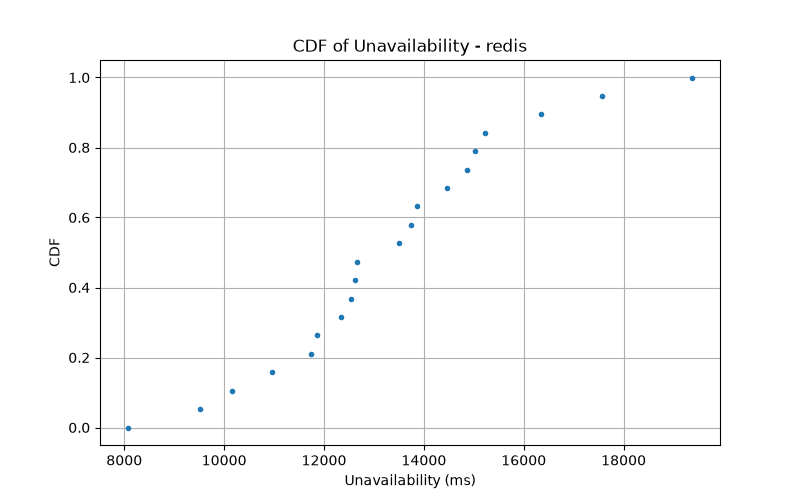
\includegraphics[width=0.95\columnwidth]{redis_cdf.png}
\caption{CDF of client-visible unavailability for Redis (AP-ish, async replication). Median = 13.08s.}
\label{fig:redis_cdf}
\end{figure}

\begin{figure}[h]
\centering
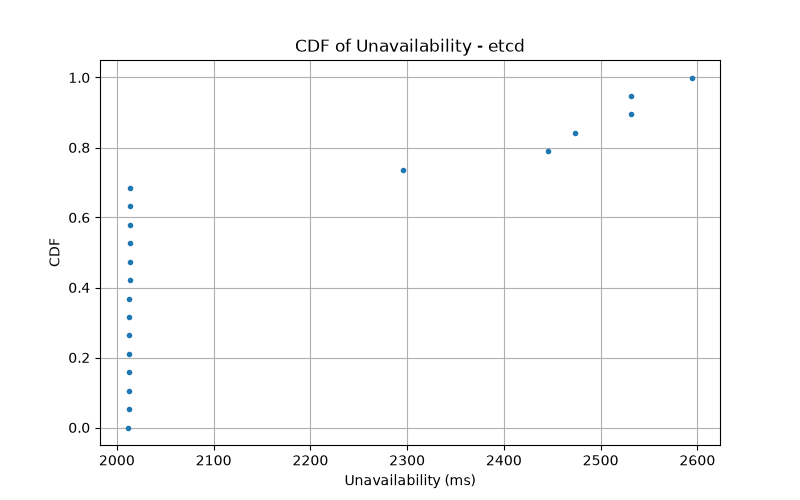
\includegraphics[width=0.95\columnwidth]{etcd_cdf_run1.png}
\caption{CDF of client-visible unavailability for etcd with aggressive timeouts (100ms/1s). Median = 2.01s, p99 = 2.58s.}
\label{fig:etcd_run1_cdf}
\end{figure}

\begin{figure}[h]
\centering
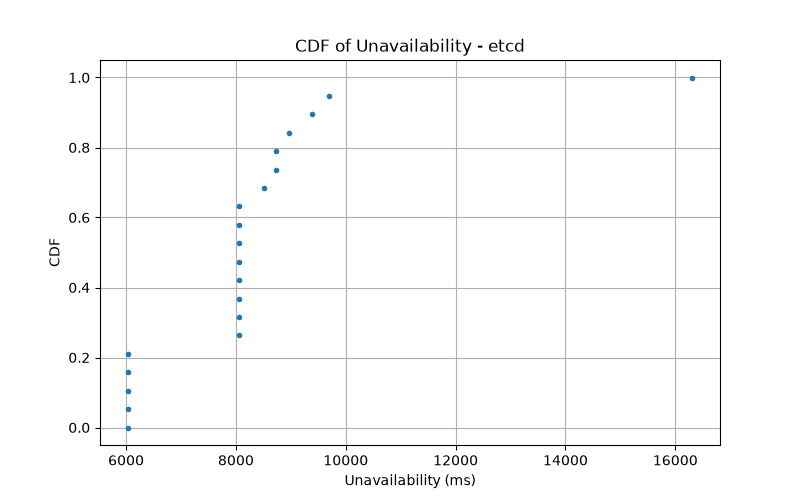
\includegraphics[width=0.95\columnwidth]{etcd_cdf_run2.png}
\caption{CDF of client-visible unavailability for etcd with conservative timeouts (500ms/5s). Median = 8.05s, p99 = 15.04s.}
\label{fig:etcd_run2_cdf}
\end{figure}

\subsection{Redis: High Median Unavailability}
Redis exhibits the highest median unavailability (13.08s). This is expected: without Sentinel, Redis performs \textit{no} automatic failover. When the master is killed, clients block until the container is restarted. The 20/20 event count confirms all kills were observed by the client. Figure~\ref{fig:redis_cdf} shows a fairly uniform distribution between 8s and 19s, reflecting the randomized recovery wait interval used in our orchestrator.

\subsection{etcd Run1: Fast Raft Election}
With aggressive timeouts (100ms/1s), etcd's median client-visible recovery is 2.01s---\textbf{6.5$\times$ faster} than Redis. More striking is the tail: p99 = 2.58s, which is \textbf{7.4$\times$ better} than Redis's p99. The election-observation time itself accounts for the bulk of this: median = 1.21s (consistent with the 1s election-timeout), p99 = 1.84s. The residual gap between election-observation time and unavailability ($\sim$0.8s) reflects the client's socket timeout and reconnection overhead.

\subsection{etcd Run2: The Cost of Conservative Tuning}
Raising the timeouts by 5$\times$ (500ms/5s) yields a median election-observation time of 6.77s and a median unavailability of 8.05s---\textbf{4$\times$ slower than Run1}. The tail degrades even more severely: unavailability p99 jumps from 2.58s to 15.04s, a \textbf{5.8$\times$ deterioration}. This super-linear tail cost is a key finding: conservative failure detection does not just shift the distribution, it widens it. Figure~\ref{fig:etcd_run2_cdf} confirms this---the CDF is noticeably less steep than that of Run1.

\subsection{Decomposing Failover Cost}
The cleanest result of this study is the direct decomposition given by
\begin{equation}
\text{Unavailability} \approx \text{Election-obs. time} + \text{Client reconnect overhead}.
\end{equation}
In Run1, Election$_{p50}$ = 1.21s and Unavailability$_{p50}$ = 2.01s (overhead $\approx$ 0.80s). In Run2, Election$_{p50}$ = 6.77s and Unavailability$_{p50}$ = 8.05s (overhead $\approx$ 1.28s). The non-electoral overhead grows modestly with longer outages but remains a small fraction of the total cost.

\section{Analysis through FLP, CAP, and Accrual Detection}

\subsection{FLP Connection}
FLP~\cite{fischer1985impossibility} establishes that no deterministic consensus protocol can guarantee both safety and liveness in an asynchronous network with even one crash. Our data confirms this at the application layer: etcd (Raft) sacrifices \textit{liveness} during elections (2--8s of unavailability), while Redis sacrifices \textit{safety} in the sense that a permanent master failure without promotion would lose acknowledged writes. Both systems coexist with FLP by accepting a trade-off.

\subsection{CAP Connection}
Under CAP, etcd is CP: during leader failure, writes are refused until a quorum elects a new leader. Redis in our setup is AP-ish: it continues serving reads/writes, but the consistency guarantee is weak (eventual at best, and only under healthy replication). The 6.5$\times$ median latency gap between them is the measurable cost of choosing C over A.

\subsection{Accrual Failure Detection}
The heartbeat-interval / election-timeout pair is precisely the suspicion threshold in $\varphi$ accrual detection~\cite{hayashibara2004phi}. Our results quantify the sensitivity-specificity trade-off with unusual clarity. A \textbf{low threshold (100ms/1s)} gives fast detection (election-observation p50 = 1.21s, p99 = 1.84s) and a tight tail, but is vulnerable to false positives under transient jitter. A \textbf{high threshold (500ms/5s)} gives slow detection (election-observation p50 = 6.77s, p99 = 9.48s) and a wider tail, but tolerates network noise.

The unavailability p99 increased by $5.8\times$ (2.58s $\rightarrow$ 15.04s), while the election-observation p99 increased by approximately $5.2\times$ (1.84s $\rightarrow$ 9.48s). This is particularly informative: increasing the suspicion threshold does \textit{not} uniformly shift recovery times; it disproportionately penalizes the tail. This is the quantitative signature of the sensitivity-specificity trade-off in failure detection.

\section{Threats to Validity}
\label{sec:threats}

\subsection{Internal Validity}
\textbf{Lost writes in Redis.} Our result of 0\% lost writes is a consequence of our experimental design: we restart the \textit{same} master container, allowing its AOF log to recover. This does \textit{not} demonstrate Redis's safety under permanent failure. A correct test of AP write loss would promote a replica manually (or via Sentinel) and compare the promoted replica's dataset against the client's log. We explicitly note that our Redis experiment measures \textit{restart recovery time}, not data-durability behavior under permanent master loss.

\textbf{Container vs.~hardware failure.} \texttt{kill -9} on a Docker container does not simulate partial network partitions, disk failures, or asymmetric latency---all of which are common in production.

\textbf{Client timeout granularity.} The 2-second socket timeout bounds our measurement precision at the lower end. A sub-second timeout (e.g., 100ms) would reveal finer-grained recovery dynamics; conversely, some Run1 kills may have been invisible to the client because the election completed before the timeout expired.

\subsection{External Validity}
\textbf{Single-host deployment.} All containers share a single physical CPU and network interface. Cross-datacenter latency, packet loss, and BGP convergence are absent.

\textbf{Small cluster.} Three-node clusters are minimal quorums. Larger clusters (5 or 7 nodes) would exhibit different election dynamics.

\textbf{Light workload.} 100 ops/s is far below production rates. Higher throughput could expose queueing effects during recovery.

\subsection{Construct Validity}
\textbf{Client-visible unavailability} conflates network delay, server unavailability, and client retry logic. A more precise metric would use monotonic clocks and separate connection-, request-, and election-level timings.

\textbf{Randomized kills} could coincidentally align with GC pauses, disk flushes, or Docker daemon events, inflating some intervals.

\subsection{Conclusion Validity}
Twenty kill events per system are sufficient to estimate p50 and (roughly) p99, but not p99.9. Given n=20, p99 corresponds approximately to the maximum observed value; percentile interpolation choices can shift p99 by up to one sample. The p99 values reported here should be interpreted as indicative, not definitive.

\section{Conclusion}
We quantified the true cost of failover in etcd and Redis under 60 total randomized kill events, with explicit decomposition into election-observation time and client-visible unavailability. Our findings are threefold: (1) CP systems recover 6.5$\times$ faster at the median than AP systems without automatic failover; (2) failure-detector tuning has a 4$\times$ impact on median recovery and a 5.8$\times$ impact on tail latency; and (3) the failover cost decomposes cleanly as election-observation time plus a small, roughly constant client-reconnect overhead. We recommend aggressive timeouts (100ms/1s) for latency-critical CP workloads, and conservative timeouts (500ms/5s) only for environments where transient network jitter would otherwise trigger spurious elections. Future work should explore Redis Sentinel for permanent-failure testing, 5-node clusters, and cross-datacenter latency.

\section*{Acknowledgment}
The author gratefully acknowledges the guidance of \textbf{Dr. Widad Al-Sarouri} (Advanced Operating Systems course, University of Science and Technology, Yemen) throughout the design and execution of this study, as well as the Department of Computer Science for providing the laboratory environment.

\begin{thebibliography}{00}
\bibitem{gilbert2002brewer} S. Gilbert and N. Lynch, ``Brewer's conjecture and the feasibility of consistent, available, partition-tolerant web services,'' \textit{ACM SIGACT News}, vol. 33, no. 2, pp. 51--59, 2002.
\bibitem{ongaro2014search} D. Ongaro and J. Ousterhout, ``In search of an understandable consensus algorithm,'' in \textit{Proc. USENIX ATC}, 2014, pp. 305--319.
\bibitem{fischer1985impossibility} M. J. Fischer, N. A. Lynch, and M. S. Paterson, ``Impossibility of distributed consensus with one faulty process,'' \textit{J. ACM}, vol. 32, no. 2, pp. 374--382, 1985.
\bibitem{hayashibara2004phi} N. Hayashibara, X. D\'efago, R. Yared, and T. Katayama, ``The $\varphi$ accrual failure detector,'' in \textit{Proc. IEEE SRDS}, 2004, pp. 66--78.
\bibitem{redis2024replication} Redis Documentation, ``Replication,'' 2024. [Online]. Available: https://redis.io/docs/management/replication/
\bibitem{chandra1996unreliable} T. D. Chandra and S. Toueg, ``Unreliable failure detectors for reliable distributed systems,'' \textit{J. ACM}, vol. 43, no. 2, pp. 225--267, 1996.
\bibitem{kleppmann2017designing} M. Kleppmann, \textit{Designing Data-Intensive Applications}. Sebastopol, CA: O'Reilly Media, 2017.
\end{thebibliography}

\end{document}